In this section, we are going to talk about UB not as it is specified by the standard and applies to C++, but as it is specified by you, the programmer, and applies to your software. To get there, it is helpful first to consider UB from a different point of view. 

All the examples of UB that we have seen so far can be divided into two kinds. The first kind is code such as ++k + k. These are bugs, since such code has no defined behavior at all. The second kind is code such as k + 1, where k is a signed integer. This code is everywhere, and most of the time, it works just fine. Its behavior is well defined except for certain values of the variables.

In other words, the code has implicit preconditions: as long as these preconditions are satisfied, the program is well behaved. Note that in the larger context of the program, these preconditions may or may not be implicit: the program may validate the inputs or intermediate results and guard against values that would cause UB. Either way, the programmer has defined a contract with the user: if the inputs obey certain restrictions, the results are guaranteed to be correct; in other words, the program behaves in a well-defined way.

What happens when the restrictions are violated?

There are the following two possibilities:

\begin{itemize}
\item 
First, the program may detect that the inputs are out of contract and handle the error. This behavior is still well defined and is a part of the specification.

\item 
Second, the program may fail to detect that the contract is violated and proceed as it usually does. Since the contract was essential to guarantee the correct result, the program now operates in uncharted territory, and there is, generally, no way to predict what is going to happen.
\end{itemize}

We just described UB.

Now that we understand that UB is simply the behavior of the program that is operating outside of the specified contract, let's think about how it applies to our software.

Most programs that are complex enough have preconditions on their inputs, a contract with the user. One could argue that these preconditions should always be checked and any errors reported. However, this can be a very expensive requirement. Again, let's consider an example.

We want to write a program that scans an image drawn on a piece of paper (or etched on a printed circuit board) and converts it to a graph data structure. The input to the program may look like this:

\hspace*{\fill} \\ %插入空行
\begin{center}
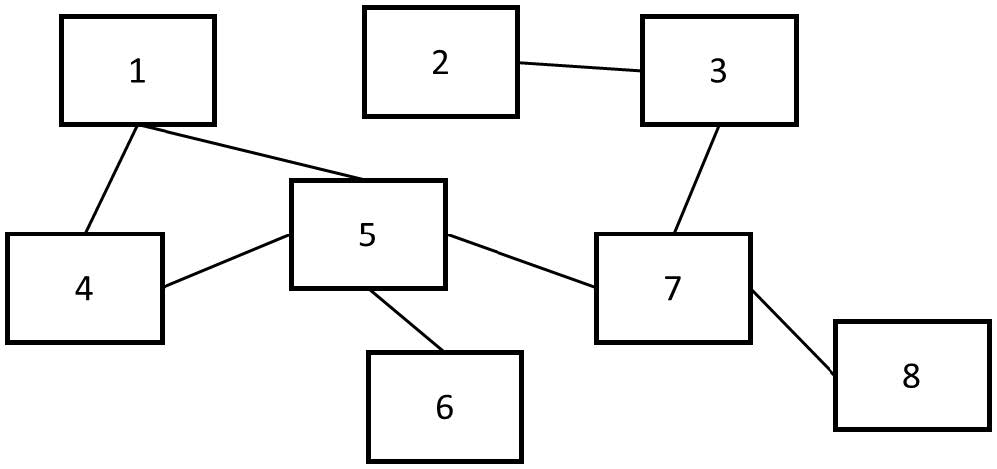
\includegraphics[width=0.9\textwidth]{content/3/chapter11/images/8.jpg}\\
Figure 11.8 – Graph drawing is an input to the graph construction program
\end{center}

The program acquires the image, recognizes rectangles, creates graph nodes from each one, recognizes the lines, for each line figures out which two rectangles it connects, and creates a corresponding edge in the graph.

Let's assume that we have an image acquisition and analysis library that gives us a set of shapes (rectangles and lines) with all their coordinates. All we have to do now is figure out which lines connect which rectangles. We have all the coordinates, so it's pure geometry from now on. One of the simplest ways to represent this graph is as a table of edges. We can use any container (say, a vector) for the table, and if we assign each node a unique numeric ID, an edge is just a pair of numbers. We can use any number of computational geometry algorithms to detect intersections between lines and rectangles and construct this table (and, with it, the graph itself) edge by edge. 

Sounds simple enough, and we have a natural representation of the data that is fairly compact and easy to work with. Unfortunately, we also have an implicit contract with the user: we ask that every line intersects exactly two rectangles (also, that rectangles do not intersect each other, but one mess at a time). 

\hspace*{\fill} \\ %插入空行
\begin{center}
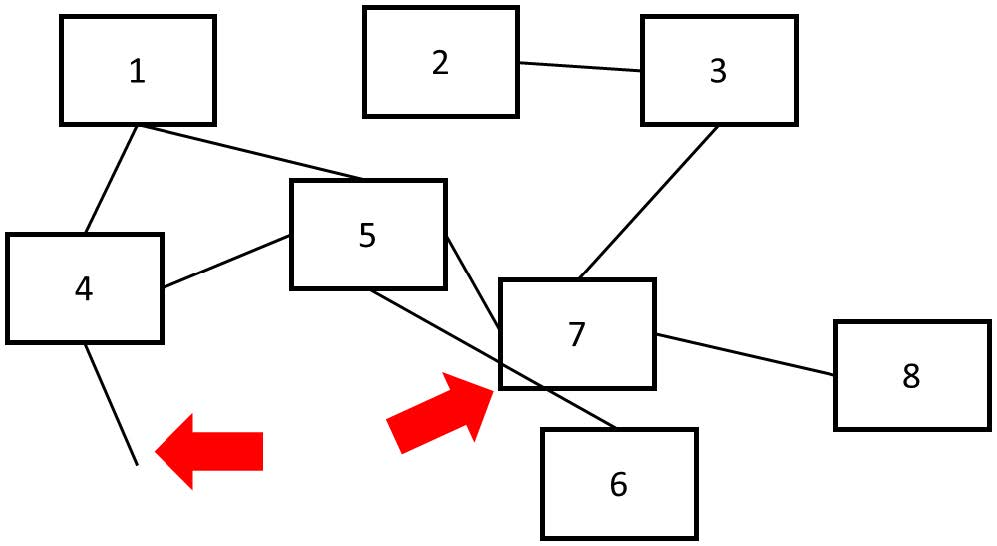
\includegraphics[width=0.9\textwidth]{content/3/chapter11/images/9.jpg}\\
Figure 11.9 – Invalid input for the graph recognition program
\end{center}

In Figure 11. 9, we see an example of input that violates the contract: one of the lines connects three rectangles, while the other touches just one. As we discussed earlier, we have two options: we can detect and report the input errors, or we can ignore them. The first option makes our program robust but carries a significant performance penalty: our original program could stop looking for rectangles connected to a given edge after it found the second such rectangle and just ignore the edge from then on. The gain from this optimization turns out to be considerable: for a graph that looks like Figure 11.8 (but much larger), it may cut the run time by half. Enforcing input validation wastes a lot of time if the input ends up being correct and frustrates the users who have other ways of ensuring that the input is valid. Not validating the input leads to UB: if we have a line connecting three rectangles, the algorithm will stop after finding the first two in whatever order it processes them (and this order may be data-dependent, so all you can really say about this situation is that an edge will be created between two of the nodes involved).

If the performance difference was insignificant (or the overall runtime was so short that doubling it doesn't matter), the best solution would be clear: validate the inputs. But in this and many other cases, validation is easily as expensive as finding the solution. What should be done in such cases?

First and foremost, we must be clear about the contract we are imposing on the user. We should clearly specify and document what constitutes a valid input. After that, the best practice for performance-critical programs is to deliver the best performance. A broader contract (the one that imposes fewer restrictions) is always better than a narrow contract, so if there are some invalid inputs we can easily detect and handle with minimal overhead, this should be done. Beyond that, all we can do is document the conditions when the behavior of the program is undefined, just like it is done in the C++ Standard. 

There is some extra effort that we can make: we can offer our users an input validation tool, either as an optional step in the program or as a separate piece of software. Running it will take time, but if the user is getting strange results from the main program, they can check to make sure the inputs are valid. This is highly preferable to simply describing when the behavior is undefined (however, there are cases where such validation is too expensive to be practical).

Wouldn't it be nice if the C++ compiler developers made the same extra effort for us, the programmers, and gave us an optional tool to detect UB in our code? As it turns out, the developers thought so too: many compilers today have an option to enable the UB sanitizer (often called UBSan). This is how it works. Let's start with some code that can result in UB:

\begin{lstlisting}[style=styleCXX]
int g(int k) {
	return k + 10;
}

\end{lstlisting}

Write a program that calls this function with a large enough argument (greater than INT\_MAX-10) and compile it with the UBSan enabled. For Clang or GCC, the option is -fsanitize=undefined. Here's an example:

\begin{tcblisting}{commandshell={}}
clang++ --std=c++17 –O3 –fsanitize=undefined ub.C
\end{tcblisting}

Run the program, and you will see something like the following:

\begin{tcblisting}{commandshell={}}
ub.C:10:20: runtime error: signed integer overflow: 
        2147483645 + 10 cannot be represented in type 'int'
\end{tcblisting}

Just like in our graph example, UB detection takes time and makes the program slower, so this is something you should do in testing and debugging. Make sanitized runs part of your regular regression testing, and do take the reported errors seriously: just because your program produces correct results today does not mean that the next compiler will not generate some very different code and change the results.

We have learned about UB, why it is sometimes a necessary evil, and how to take advantage of it to improve performance. Before you flip the page, let's recap what we have learned.

























